\section{Herleitung der Methode} \label{sec:herleitungdermethode}
Um herauszufinden, welche Linterregeln aus dem Spectral \acs{OAS} Regelwerk relevant sind, soll ein Softwaretool erstellt werden, das zuverlässig und reproduzierbar Linterfehler für die gegebenen OpenAPI Spezifikationen generiert und analysiert. In Teilen kann dabei auf die Methodik der vergleichbaren Studien zurückgegriffen werden. Zur Erhebung der Anforderungen wird die Methodik von \parencite{bergsmann_requirements_2023} verwendet. Zur Planung und Dokumentation der Softwarearchitektur wird die Methodik von \parencite{starke_effektive_2024} verwendet. Der vollständige Quellcode dieser Arbeit steht zur Verfügung\footnote{Siehe den Quellcode auf Github unter \href{https://www.github.com/paulbrenker/thesis}{https://www.github.com/paulbrenker/thesis} oder auf der beiliegenden CD.}. In diesem Kapitel wird beschrieben, wie das System konzipiert, entworfen und entwickelt wurde.


\subsection{Use Cases} \label{sec:usecases}
Im ersten Schritt wird modelliert, wie mit dem System aus Benutzersicht interagiert wird. Für die Benutzung des entworfenen Systems ist lediglich eine Nutzerkategorie notwendig, die das System und die Komponenten triggert. Alle Use Cases werden textuell \parencite{bergsmann_requirements_2023} und mithilfe von \acf{UML} Use Case Diagrammen dokumentiert \parencite{rupp_uml_2012}.

Diese Interaktionen werden in den folgenden Unterkapiteln gezeigt.


\subsubsection{Linting} \label{linting}
Den APIs.guru Datensatz mit dem Spectral \acs{OAS} Datensatz zu linten, ist die erste Benutzer Interaktion mit dem System.

\begin{longtable}{lp{0.5\linewidth}}
  \caption{\textbf{UC-1} Linting textuell.}
  \endfirsthead
  \endhead
  \hline\hline
  \textbf{Use Case} & \textbf{UC-1} \\
  \textbf{Use Case Name} & Linting \\
  \textbf{Ziel (Kundennutzen)} & Ermitteln der Linterfehler die auf allen OpenAPI Spezifikationen in im OpenAPI Directory von APIs.guru geworfen werden. \\
  \textbf{Kategorien} & Interaktion mit externen Systemen.  \\
  \textbf{Vorbedingung} & Benutzer startet den Linting Prozess über das Terminal. \\
  \textbf{Nachbedingung} & Linterfehler zu allen OpenAPI Spezifikationen des OpenAPI Directories sind lokal gespeichert. \\
  \textbf{Akteure} & USER \\
  \textbf{Trigger} & User Befehl \\
  \textbf{Standardszenario} & 
  \vspace{-0.7cm}
  \begin{enumerate}
    \item Die Pfade zu den OpenAPI Spezifikationen aus dem OpenAPI Directory werden gelesen.
    \item Der Spectral Linter wird für jede Spezifikation aufgerufen und die geworfenen Linterfehler werden gespeichert.
    \item Die Linterfehler werden auf ein speicherbares Format abgebildet.
    \item Die Linterfehler von allen Spezifikationen werden im \acf{CSV} Datenformat physisch gespeichert.
  \end{enumerate}
  \\
  \textbf{Erweiterungsszenario} & 
  \vspace{-0.7cm}
  \begin{itemize}
    \item Falls eine Spezifikation manuell als unlintbar markiert wurde, wird diese vom Linten ausgeschlossen.
  \end{itemize}
  \\
  \textbf{Risiko} & \hspace{0.8cm} gering \\
  \textbf{Qualitätsanforderungen} & 
  \vspace{-0.7cm}
  \begin{itemize}
    \item die angegebenen Szenarien können erfolgreich ausgeführt werden (Funktionalität).
    \item \textbf{QR-2} Muss bei mehrmaliger Ausführung die gleichen Ergebnisse erzeugen.
  \end{itemize}
   \\ \hline\hline
\end{longtable}

\begin{figure}[htbp]
  \centering
  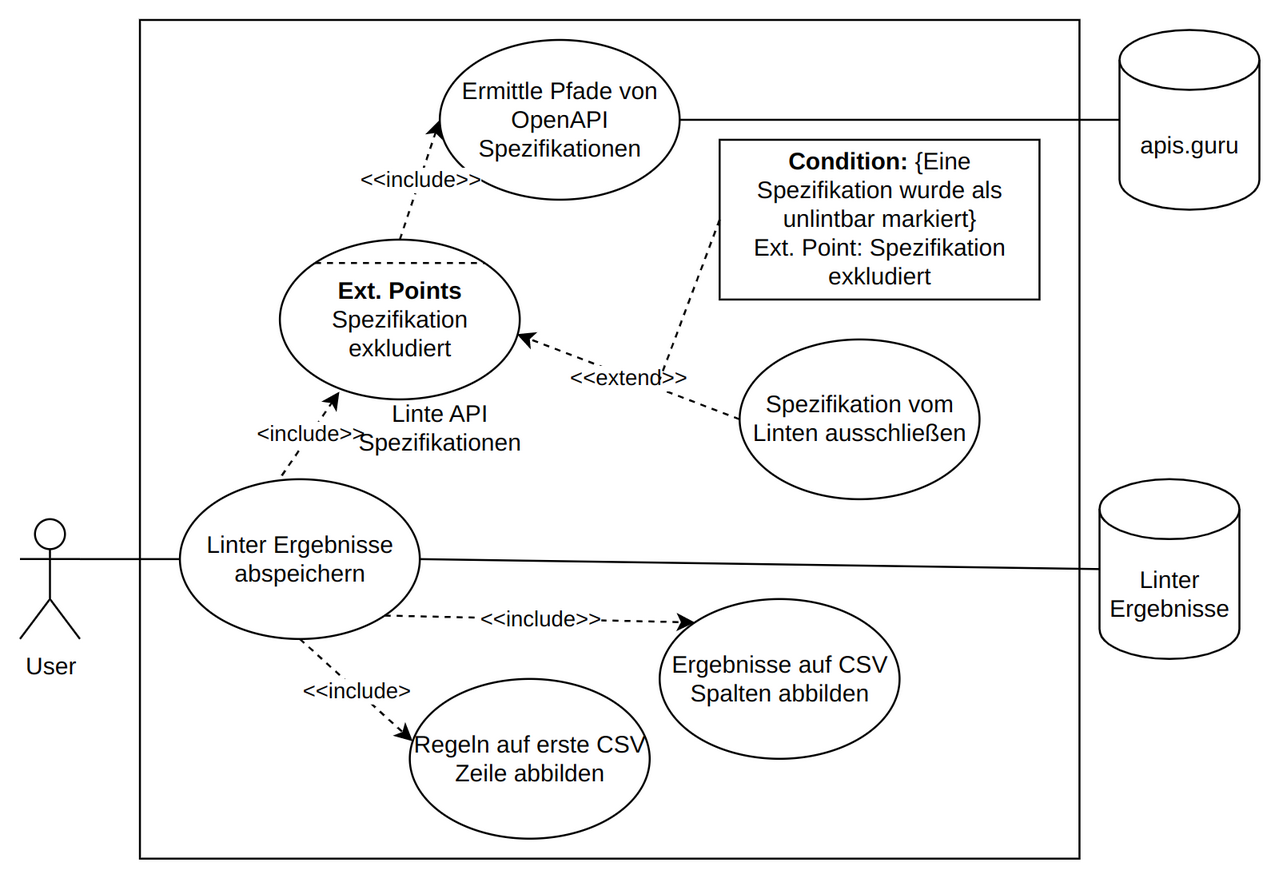
\includegraphics[width=1\linewidth]{img/linting.png}
  \caption{\textbf{UC-1} Linting Use Case Diagramm.}
  \label{fig:UC1}
\end{figure}


\subsubsection{Invertierung} \label{sec:invertierung}
Die geworfenen Linterfehler zu invertieren bedeutet, herauszufinden wie häufig eine Regel geworfen werden könnte. Die Invertierung definieren wir als die relative Anzahl der Fälle, in denen eine Regel eingehalten wurde. Es ist wichtig diese Werte zu berechnen, um Aussagen über die Relevanz treffen zu können. In diesem Use Case wird zwischen vier Klassen von Linterregeln unterschieden. Diese sollen die Größenordnung der möglichen Linterfehler anzeigen. Um die Linterregeln des \acs{OAS} Regelwerks zu klassifizieren, wird eine manuelle Analyse des Quellcodes des Regelwerkes vorgenommen.

\begin{enumerate}
  \item \textbf{Inkompatibel:} Eine Regel ist dann inkompatibel, wenn sie für \acs{OAS} Versionen spezifiziert ist, die im OpenAPI Directory von APIs.guru nicht vorkommen. Im Datensatz werden alle Spezifikationen auf \acs{OAS} 3.0 konvertiert. Folglich sind alle Versionen $v$ mit $v \neq 3.0$ inkompatibel. Auf inkompatible Regeln wird im Verlauf der Arbeit nicht weiter eingegangen.
  \item \textbf{Single Trigger:} Als Single Trigger gelten Regeln, die pro Spezifikation maximal ein Mal ausgelöst werden können.
  \item \textbf{Multi Trigger:} Diese Regeln können mehrmals in einer Spezifikation geworfen werden.
  \item \textbf{Multi Message:} Multi Message Regeln können mehrmals pro Spezifikation geworfen werden. Für jede gelintete Stelle können mehrere Arten von Linterfehlern geworfen werden.
\end{enumerate} 

\begin{longtable}{lp{0.5\linewidth}}
  \caption{\textbf{UC-2} Invertierung textuell.}
  \endfirsthead
  \endhead
  \hline\hline
  \textbf{Use Case} & \textbf{UC-2} \\ 
  \textbf{Use Case Name} & Invertierung \\
  \textbf{Ziel (Kundennutzen)} & Ermitteln der Anzahl der Linterfehler, die pro Linterregel auf einer Spezifikation ausgelöst werden könnten. \\
  \textbf{Kategorien} & Erstellen von Metadaten \\
  \textbf{Vorbedingung} & Mögliche Linterfehler für die OpenAPI Spezifikationen wurden ermittelt. \\
  \textbf{Nachbedingung} & Metadaten zu den Inversen liegen in Form einer \acs{CSV} Datei vor. \\
  \textbf{Akteure} & USER \\
  \textbf{Trigger} & User Befehl \\
  \textbf{Standardszenario} & 
  \vspace{-0.7cm}
  \begin{itemize}
    \item Rufe für jede OpenAPI Spezifikation und für jede Regel die Invertierung auf.
  \end{itemize}
  \\
  \textbf{Erweiterungsszenario} & 
  \vspace{-0.7cm}
  \begin{enumerate}
    \item Wenn eine Regel inkompatibel ist, werden diese ignoriert.
    \item Wenn eine Regel eine Single Trigger Regel ist, ist dies die maximal mögliche Anzahl der Auslösungen.
    \item Wenn eine Regel eine Multi Trigger Regel ist, gib die Anzahl der möglichen Auslösungen zurück.
    \item Wenn eine Regel eine Multi Message Regel ist, gebe die Anzahl der möglichen Auslösungen zurück.
  \end{enumerate}
  \\
  \textbf{Risiko} & \hspace{0.8cm} hoch \\
  \textbf{Qualitätsanforderungen} & 
  \vspace{-0.7cm}
  \begin{itemize}
    \item Das angegebene Standardszenario und die Erweiterungsszenarien können erfolgreich ausgeführt werden (Funktionalität).
    \item \textbf{QR-2} Muss bei mehrmaliger Ausführung die gleichen Ergebnisse erzeugen.
  \end{itemize}
   \\ \hline\hline
\end{longtable}
\begin{figure}[htbp]
  \centering
  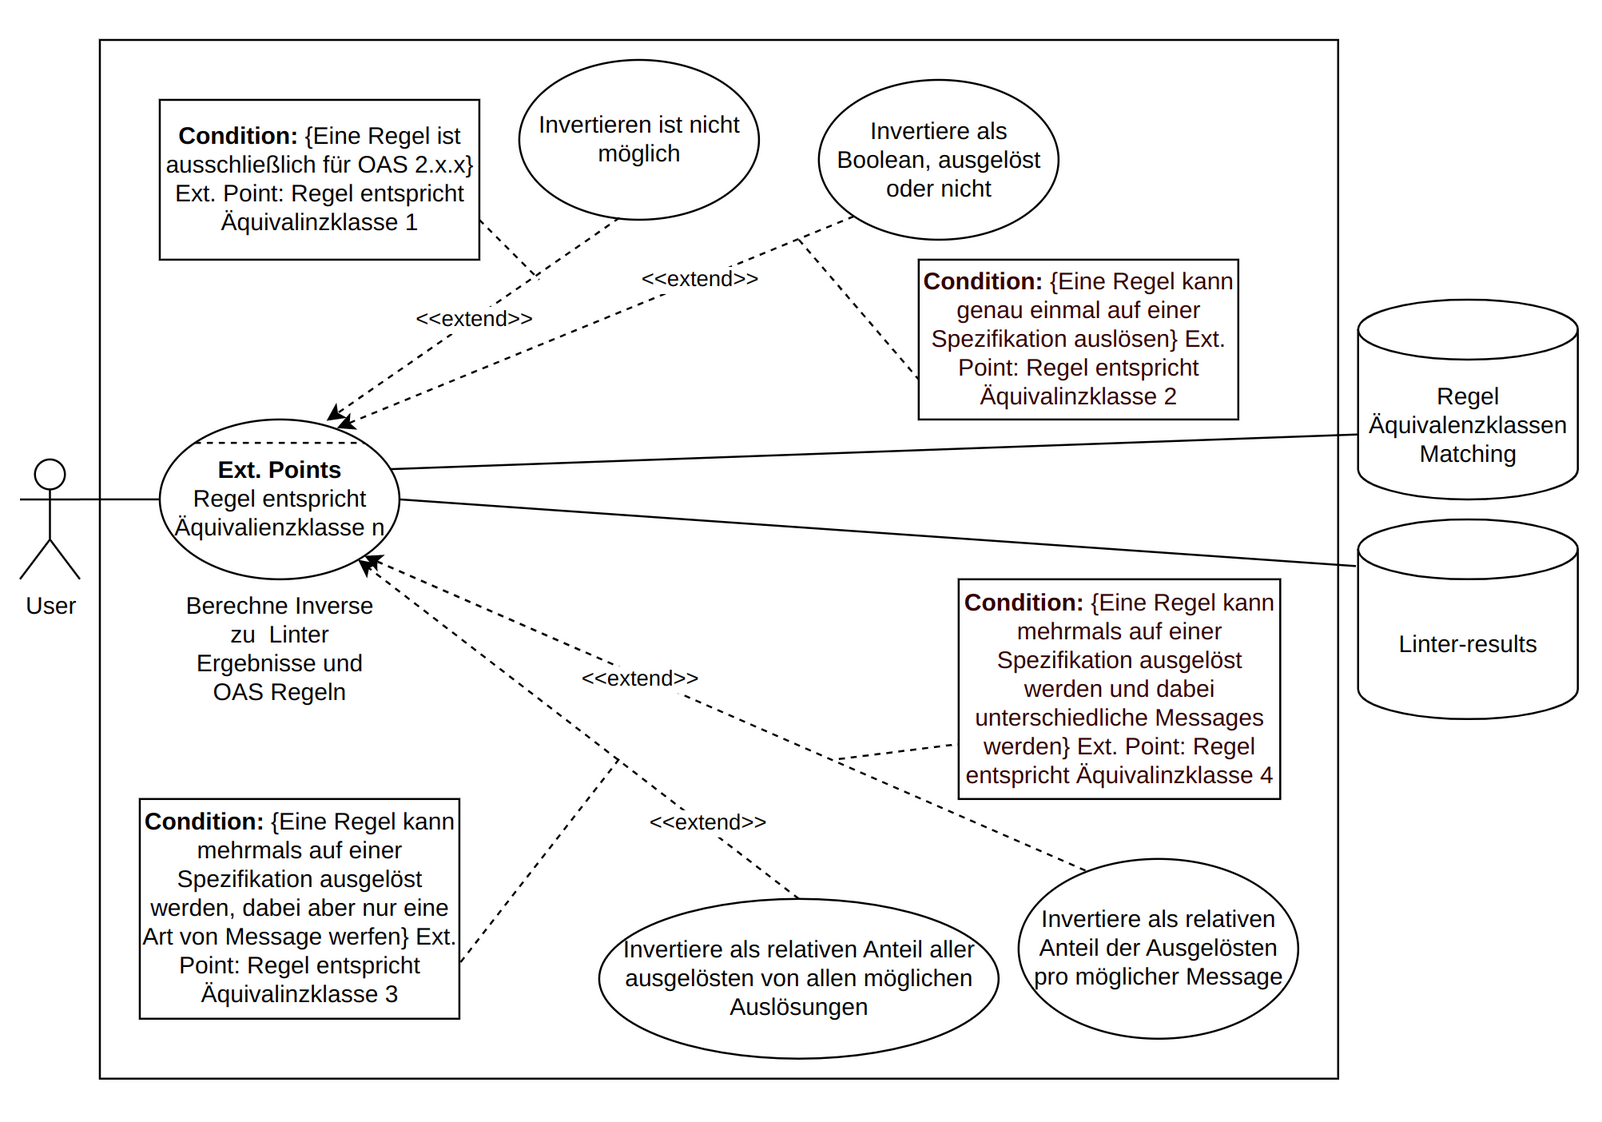
\includegraphics[width=1\linewidth]{img/invert.png}
  \caption{\textbf{UC-2} Invertierung von Linterfehlern}
  \label{fig:UC2}
\end{figure}

\newpage
Es wird eine Strategie verwendet, die für alle Regeln mögliche Selektionen ermittelt, an denen die Regel ausgelöst werden könnte. Der Algorithmus für die Strategie ist in Algorithmus \ref{alg:invert} als Pseudocode angegeben. Dies verdeutlicht die Funktionalität dieses Aspektes der Software. Aus dem given Objekt einer Spectral Regel werden die JSONPath\footnote{JSONPath ist eine deklarative Abfragesprache, \acs{JSON} Werte und Objekte zu selektieren und zu extrahieren \parencite{friesen_extracting_2019}} Objekte gelesen. Das Ergebnis einer Anwendung eines JSONPath auf ein \acs{JSON} Objekt ist ein Array an selektierten Teilobjekten. Die Länge dieses Arrays entspricht den möglichen Selektionen des JSONPaths und damit den möglichen Linterfehlern. Die Länge aller JSONPaths einer Linterregel werden aufsummiert und zurückgegeben.

\begin{algorithm}
  \caption{Ermitteln der möglichen Stellen für Linterfehler}
  \label{alg:invert}
  \textbf{Eingabe:} Spezifikation, Linterregel \\
  \textbf{Ausgabe:} Anzahl möglicher Stellen
\begin{algorithmic}[1]
    \State \textit{summe}: Int := 0
    \State \textit{given}: List(JSONPath) := Linterregel.\textit{given}
    \For{each \textit{element}: JSONPath in \textit{given}}
        \State \textit{pfade}: Liste := JSONPath.apply(Spezifikation, \textit{element})
        \State \textit{länge}: Int := \textit{pfade}.length()
        \State \textit{summe} += \textit{länge}
    \EndFor
    \State \Return \textit{summe}
\end{algorithmic}
\end{algorithm}


\subsubsection{Analyse} \label{sec:analyse}
Die Benutzerinteraktion mit der Datenanalyse Software Pipeline findet nach den in \textbf{UC-1} und \textbf{UC-2} beschriebenen Interaktionen statt. Zweck dieser Interaktion ist es, die ermittelten Linterfehler und die Metadaten in ein menschenlesbares Format zu bringen und sie im Rahmen eine \acf{EDA} zu beschreiben. 

\begin{longtable}{lp{0.5\linewidth}}
  \caption{\textbf{UC-3} Analyse textuell.}
  \endfirsthead
  \endhead
  \hline\hline
  \textbf{Use Case} & \textbf{UC-3} \\ 
  \textbf{Use Case Name} & Analyse \\
  \textbf{Ziel (Kundennutzen)} & \acs{EDA} und Clusteranalyse der Linter- und Invertierungsdaten. \\
  \textbf{Kategorien} & Datenvisualisierung \\
  \textbf{Vorbedingung} & Interaktionen \textbf{UC-1} und \textbf{UC-2} abgeschlossen. \\
  \textbf{Nachbedingung} & Visualisierungen und tabellenartige Darstellung von Daten liegt vor. \\
  \textbf{Akteure} & USER \\
  \textbf{Trigger} & User Befehl \\
  \textbf{Standardszenario} & 
  \vspace{-0.7cm}
  \begin{enumerate}
    \item Die Daten werden auf das benötigte Format abgebildet.
    \item Je nach Spezifikation der Analyse wird eine tabellarische Übersicht (Erweiterungsszenario 1) oder ein Plot (Erweiterungsszenario 2) erstellt.
    \item Erstellte Übersichten werden gespeichert: Plots unter tex/thesis/img und Tabellen unter data/analysis-results.
  \end{enumerate}
  \\
  \textbf{Erweiterungsszenario} & 
  \vspace{-0.7cm}
  \begin{enumerate}
    \item Aggregiere die Daten zu einer Tabelle mit Linterregeln in der ersten Spalte.
    \item Aggregiere die Daten und erstelle einen Plot mit Linterregeln auf der x-Achse.
  \end{enumerate}
  \\
  \textbf{Risiko} & \hspace{0.8cm} mittel \\
  \textbf{Qualitätsanforderungen} & 
  \vspace{-0.7cm}
  \begin{itemize}
    \item Das angegebene Standardszenario und die Erweiterungsszenarien können erfolgreich ausgeführt werden (Funktionalität).
    \item \textbf{QR-2} Muss bei mehrmaliger Ausführung die gleichen Ergebnisse erzeugen.
    \item \textbf{QR-6} Alle Plots müssen mit Grid, Labels und Achsenbeschriftungen versehen werden.
  \end{itemize}
   \\ \hline\hline
\end{longtable}
\begin{figure}[htbp]
  \centering
  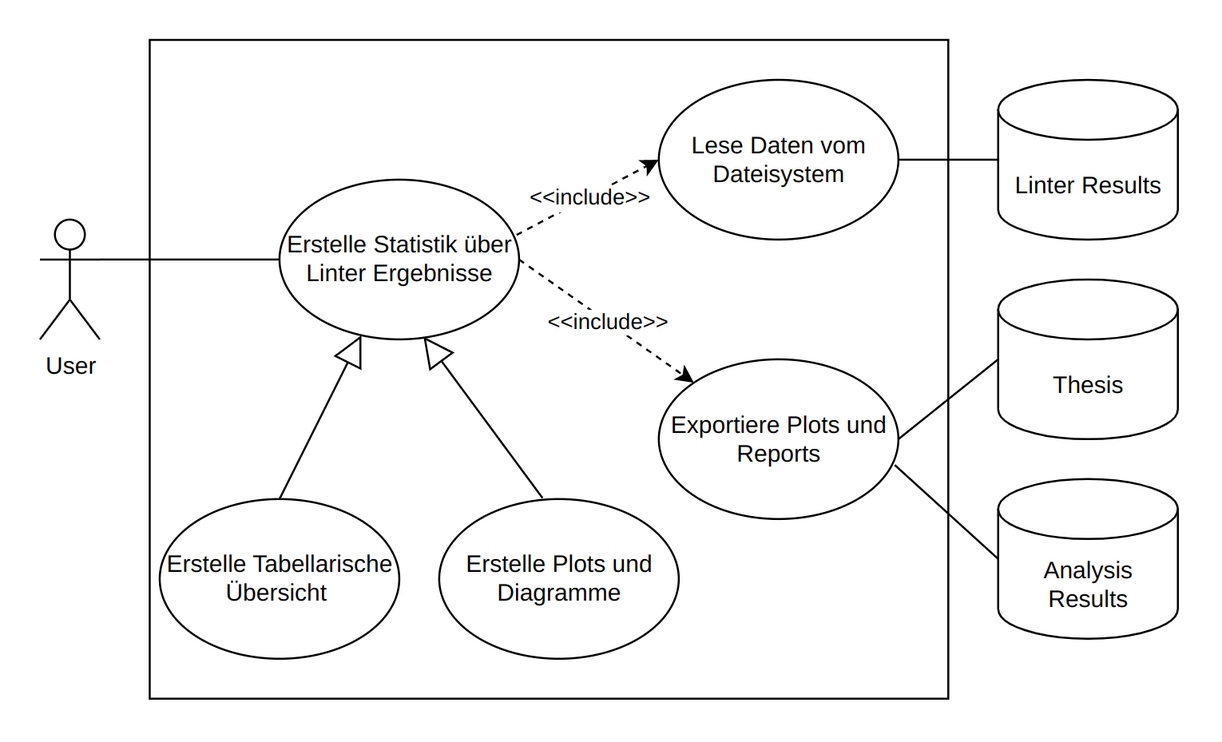
\includegraphics[width=1\linewidth]{img/describe.png}
  \caption{\textbf{UC-3} Analyse der ermittelten Daten}
  \label{fig:UC3}
\end{figure}


\subsection{Anforderungen} \label{sec:anforderungen}
Zusätzlich zu den vorgeschriebenen Interaktionen werden Anforderungen für das System formuliert. Die Formulierung von Anforderungen hilft dabei, alle relevanten Aspekte zu berücksichtigen \parencite{bergsmann_requirements_2023}.

Die Anforderungen werden unterteilt in funktionale Anforderungen, Qualitätsanforderungen und Einschränkungen. Anforderungen werden textuell nach dem Vorbild der Anforderungsschablonen aus dem SOPHIST Regelwerk \parencite{rupp_requirements-engineering_2014} formuliert.


\subsubsection{Funktionale Anforderungen} \label{sec:funktionaleanforderungen}
\begin{itemize}
  \item \textbf{FR-1} Die Software sollte eine kommandozeilenbasierte Interaktion für das Starten des Tools und der Datenanalysepipeline bereitstellen.
  \item \textbf{FR-2} Die Software muss die Verzeichnisstruktur des OpenAPI Directory von APIs.guru scannen und OpenAPI Spezifikationen finden können.
  \item \textbf{FR-3} Die Software muss den Spectral \acs{API} Linter und das Spectral \acs{OAS} Regelwerk verwenden, um den APIs.guru Datensatz zu linten.
  \item \textbf{FR-4} Die Software muss die JSONPath-plus Bibliothek verwenden, um Invertierungen zu berechnen.
  \item \textbf{FR-5} Die Software muss Dateien im \acs{CSV} Format nach \texttt{data/linter-results} speichern.
  \item \textbf{FR-6} Die Software muss Linterergebnisse \acs{CSV} lesen können und anhand von Abfragen, Zeilen einschränken, Spalten einschränken und Zellinhalte auf berechnete Werte abbilden können.
  \item \textbf{FR-7} Die Software muss Plots und Abbildungen der Datenanalyse direkt im Verzeichnis \texttt{tex/thesis/img} speichern.
\end{itemize}


\subsubsection{Qualitätsanforderungen} \label{sec:qualitätsanforderungen}
\begin{itemize}
  \item \textbf{QR-1} Das Softwaretool sollte während des Lintings und der Invertierung einen Fortschrittsbalken anzeigen.
  \item \textbf{QR-2} Alle Systemteile müssen bei mehrmaliger Ausführung immer die gleichen Ergebnisse erzeugen.
  \item \textbf{QR-3} Das Softwaretool sollte für die Berechnung der Linterfehler und Inversen auf Parallelisierung zurückgreifen.
  \item \textbf{QR-4} Das Softwaretool sollte Dateien mit Linter Ergebnissen und Datenanalyse Ergebnissen mit dem Datum und dem aktuellen Committag bezeichnen. Das hilft dabei, Ergebnisse zu reproduzieren.
  \item \textbf{QR-5} Alle Systemteile sollten mit Unit-Tests versehen werden. Die Testabdeckung sollte dabei nicht geringer als 80 \% sein.
  \item \textbf{QR-6} Alle Plots müssen mit einem Grid, Labels und Beschriftungen für x- und y-Achse versehen werden. 
\end{itemize}


\subsubsection{Einschränkungen} \label{sec:einschränkungen}
\begin{itemize}
  \item \textbf{C-1} Die Software für den Linting und Invertierungsprozess muss in JavaScript oder TypeScript entwickelt werden, um die volle Funktionalität der Spectral Bibliotheken zu garantieren und, um die gleiche Implementierung von JSONPath zu verwenden.
  \item \textbf{C-2} Die Software sollte ausschließlich mit \acs{YAML} Dateien operieren können. Das schließt Fehler mit falsch gelesenen Dateien aus.
  \item \textbf{C-3} Die Datenanalyse sollte mit Python, Pandas und Matplotlib implementiert werden. Diese bieten viele moderne Methoden zur Datenanalyse.
\end{itemize}


\subsection{Software Architektur} \label{sec:softwarearchitektur}
In diesem Abschnitt werden der Entwurfsprozess und die Entwurfsentscheidungen für die im Rahmen dieser Arbeit entwickelte Software dokumentiert. In diesem Prozess wurden die vorgegebenen Interaktionen und Anforderungen berücksichtigt. Die gezeigten vier Sichten nach \parencite{starke_effektive_2024} sollen die Softwarearchitektur effektiv und bedarfsgerecht beschreiben. Die Dokumentation enthält damit auch die Kernelemente der Architekturdokumentation nach der Arc42 Vorlage\footnote{Arc42 ist eine Vorlage (Template) mit einer strukturierten Methode für die Dokumentation von Software und Systemarchitekturen. Arc42 wurde von P. Hruschka und G. Starke entwickelt und steht unter \href{https://www.arc42.de/}{https://www.arc42.de/} online zur Verfügung.} \parencite{starke_arc42_2024}.


\subsubsection{Kontextsicht} \label{sec:kontextsicht}
Die Kontextsicht zeigt, wie ein System in seine Umgebung eingebettet ist und welche Schnittstellen zu Nachbarsystemen vorhanden sind \parencite{starke_effektive_2024}. Für das hier entwickelte Softwaresystem ist die wichtigste Schnittstelle nach außen die Verwendung des OpenAPI Directory von APIs.guru. Eine weitere Schnittstelle, die für die Funktionalität des Systems wichtig ist, ist die Verwendung des Spectral \acs{API} Linters und des Spectral OAS Regelwerks, die hier als Software Bibliotheken eingebunden werden können. Weiterhin kann die Kontextsicht den Datenfluss zwischen den Softwarekomponenten zeigen. Die Analyse Pipeline und das Tool zum Linten der Spezifikationen werden als zwei unabhängige Komponenten entwickelt. Die Datenanalyse kann auf Ergebnisse des Linter Tools über das Dateisystem zugreifen.

\begin{figure}[htbp]
  \centering
  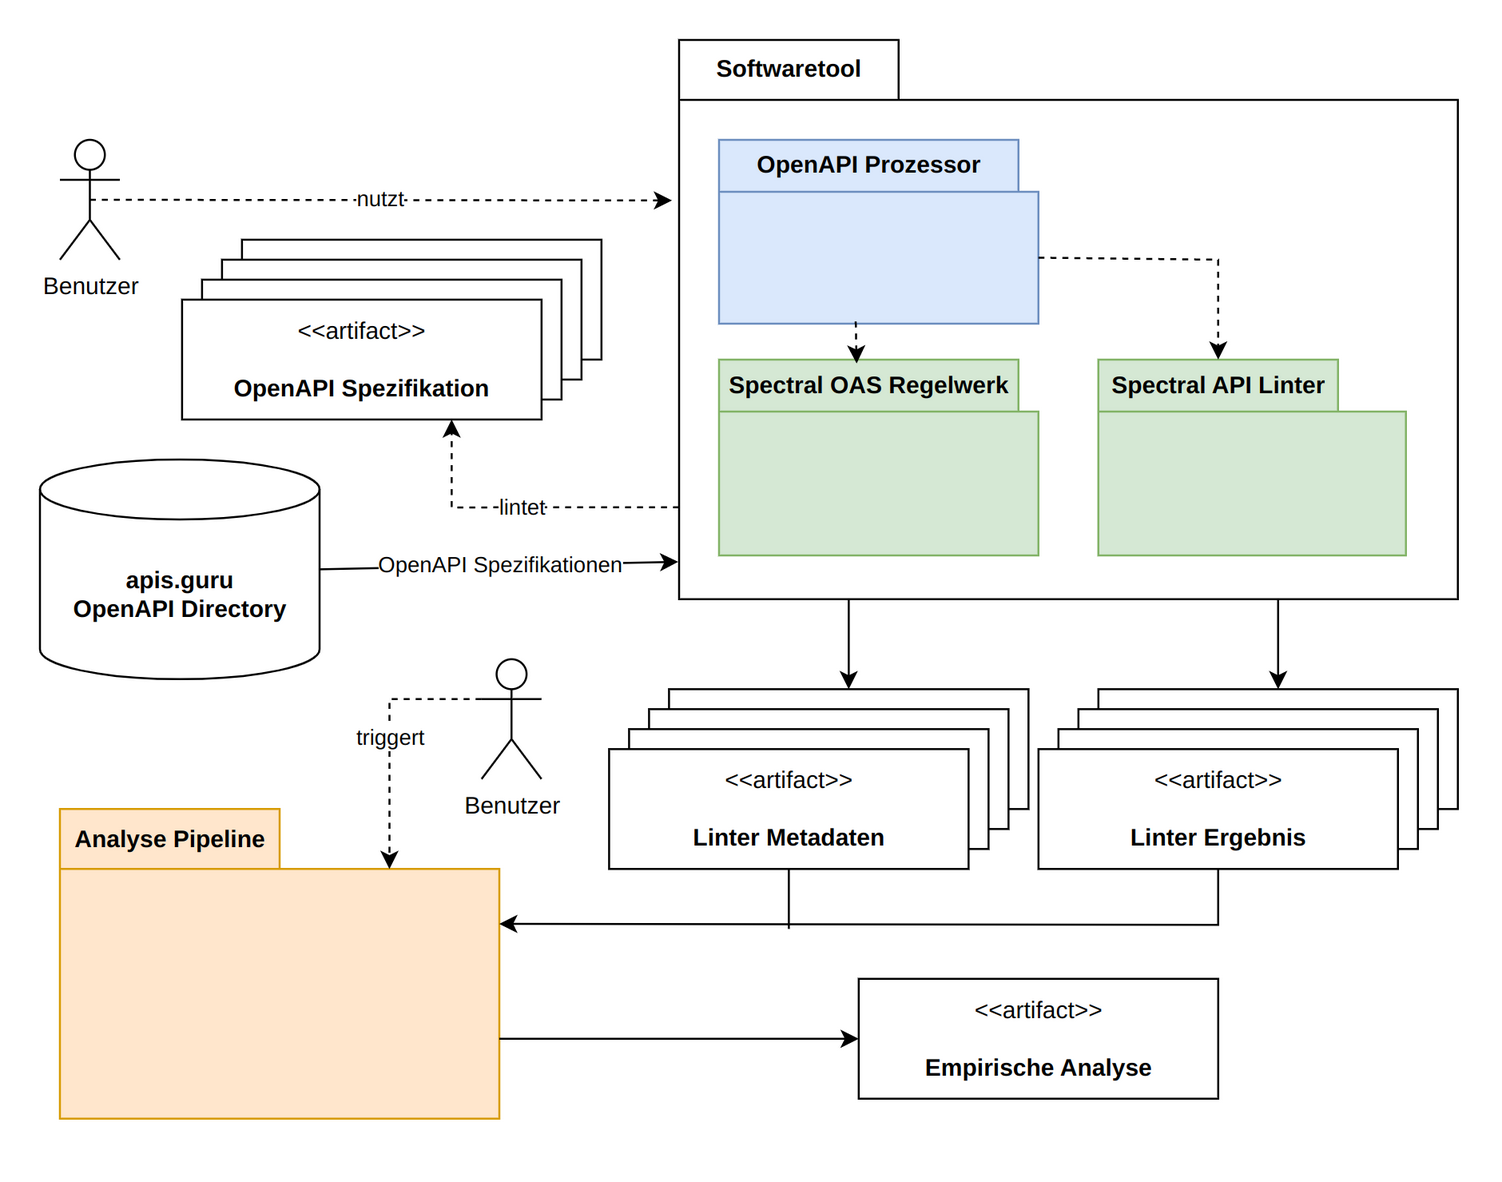
\includegraphics[width=1\linewidth]{img/contextview.png}
  \caption{Kontextsicht des Systems}
  \label{fig:Kontextsicht}
\end{figure}

\newpage
\subsubsection{Bausteinsicht} \label{sec:bausteinsicht}
Die Bausteinsicht zeigt, wie ein System intern aufgebaut ist und wie das Code Repository strukturiert ist, \parencite{starke_effektive_2024}. Es wird Top Down dokumentiert, welche Bausteine auf den verschiedenen Levels zum Einsatz kommen. Die einzelnen Bausteine werden als Whiteboxes gezeigt, die die darunterliegende Struktur und damit auch die Paketzerlegung des Quellcodes verdeutlichen. Die Bausteine zeigen den Teil des Code Repositorys, der die funktionalen Anforderungen implementiert. In den Levels werden Bausteine des Systems aufgebrochen und im Detail beschrieben. Die Technologien, auf denen die Komponenten Lintertool und Datenanalyse aufbauen, sind sichtbar. In der untersten Schicht sind Schlüssel Abhängigkeiten erwähnt, die für die Anforderungen notwendig sind.

Das Lintertool läuft in einer Node.js Umgebung und ist in TypeScript implementiert. Der Code wird mit dem tsc Compiler kompiliert und Module werden mit dem node package manager (npm) verwaltet. 

Die Datenanalysepipeline läuft in einer python3 Umgebung. Die eingebundenen Module werden mit dem Tool poetry verwaltet.

\begin{figure}[htbp]
  \centering
  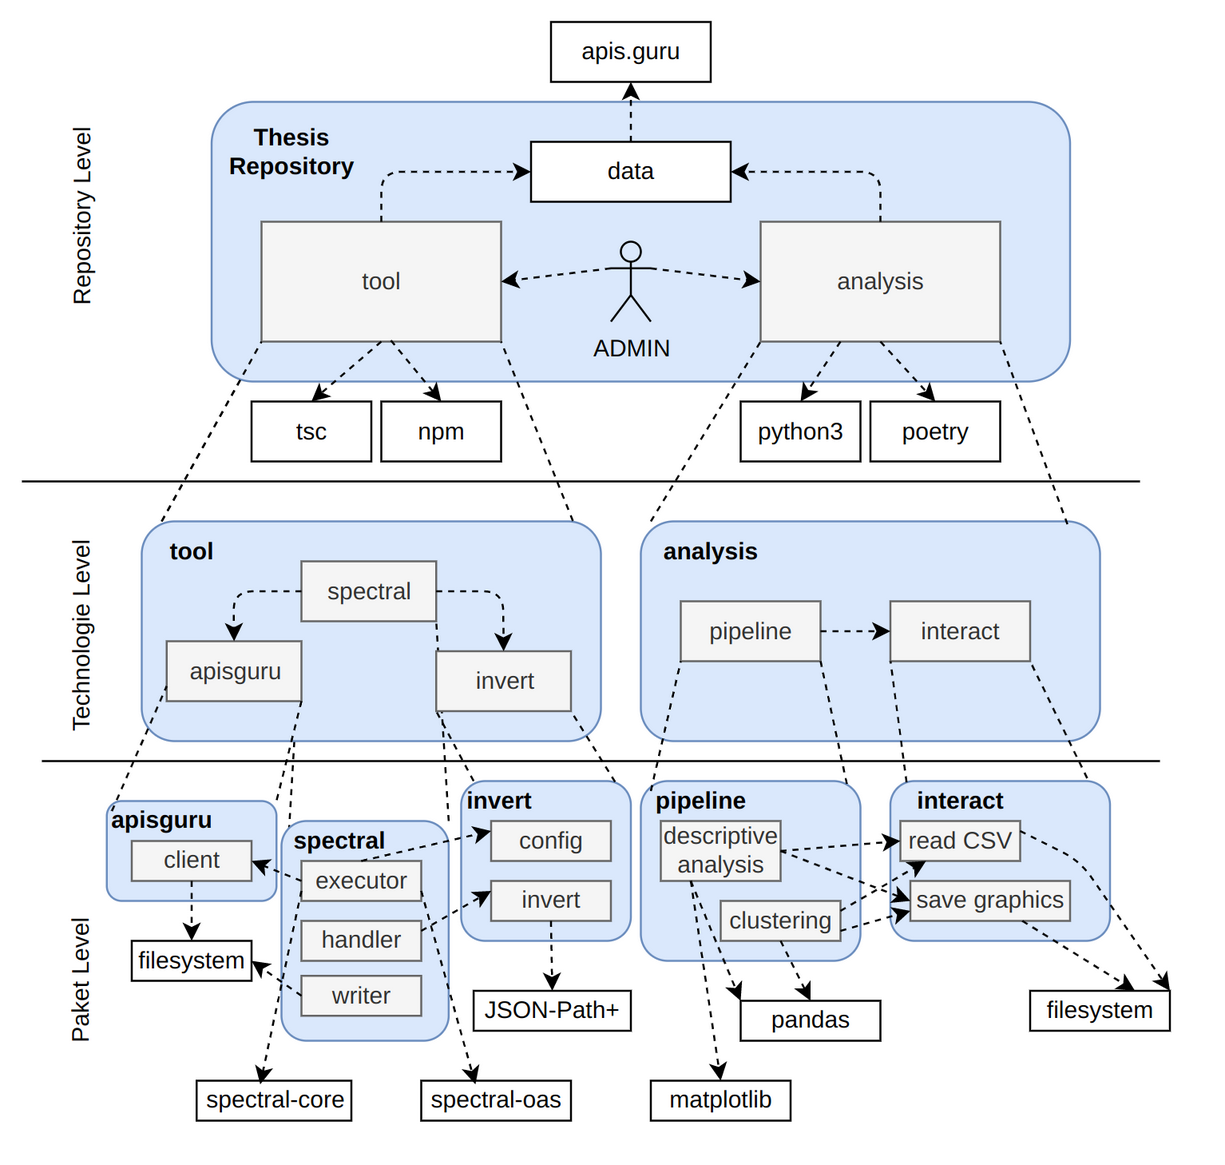
\includegraphics[width=1\linewidth]{img/buildingblockview.png}
  \caption{Bausteinsicht des Systems}
  \label{fig:Bausteinsicht}
\end{figure}


\subsubsection{Laufzeitsicht} \label{sec:laufzeitsicht}
Die Laufzeitsicht zeigt die Zusammenwirkung von wichtigen Bausteinen des Systems zur Laufzeit \parencite{starke_effektive_2024}. Hier wird die zeitliche Abfolge von Methodenaufrufen und dynamischen Interaktionen dokumentiert. Insbesondere ist hier zu sehen, wie die OpenAPI Spezifikationen aus dem OpenAPI Directory iterativ verarbeitet werden und dabei in Folge mehrere Funktionen aufgerufen werden.  Die mit loop gekennzeichnete Schleife zeigt die Kernfunktionalität des Linter Tools.

Eine Laufzeitsicht für die Datenanalyse liefert hier keinen Erkenntnisgewinn. Die Methodik zur Datenanalyse ist im Kapitel \ref{chapter:dataanalysis} Datenanalyse beschrieben.

\begin{figure}[htbp]
  \centering
  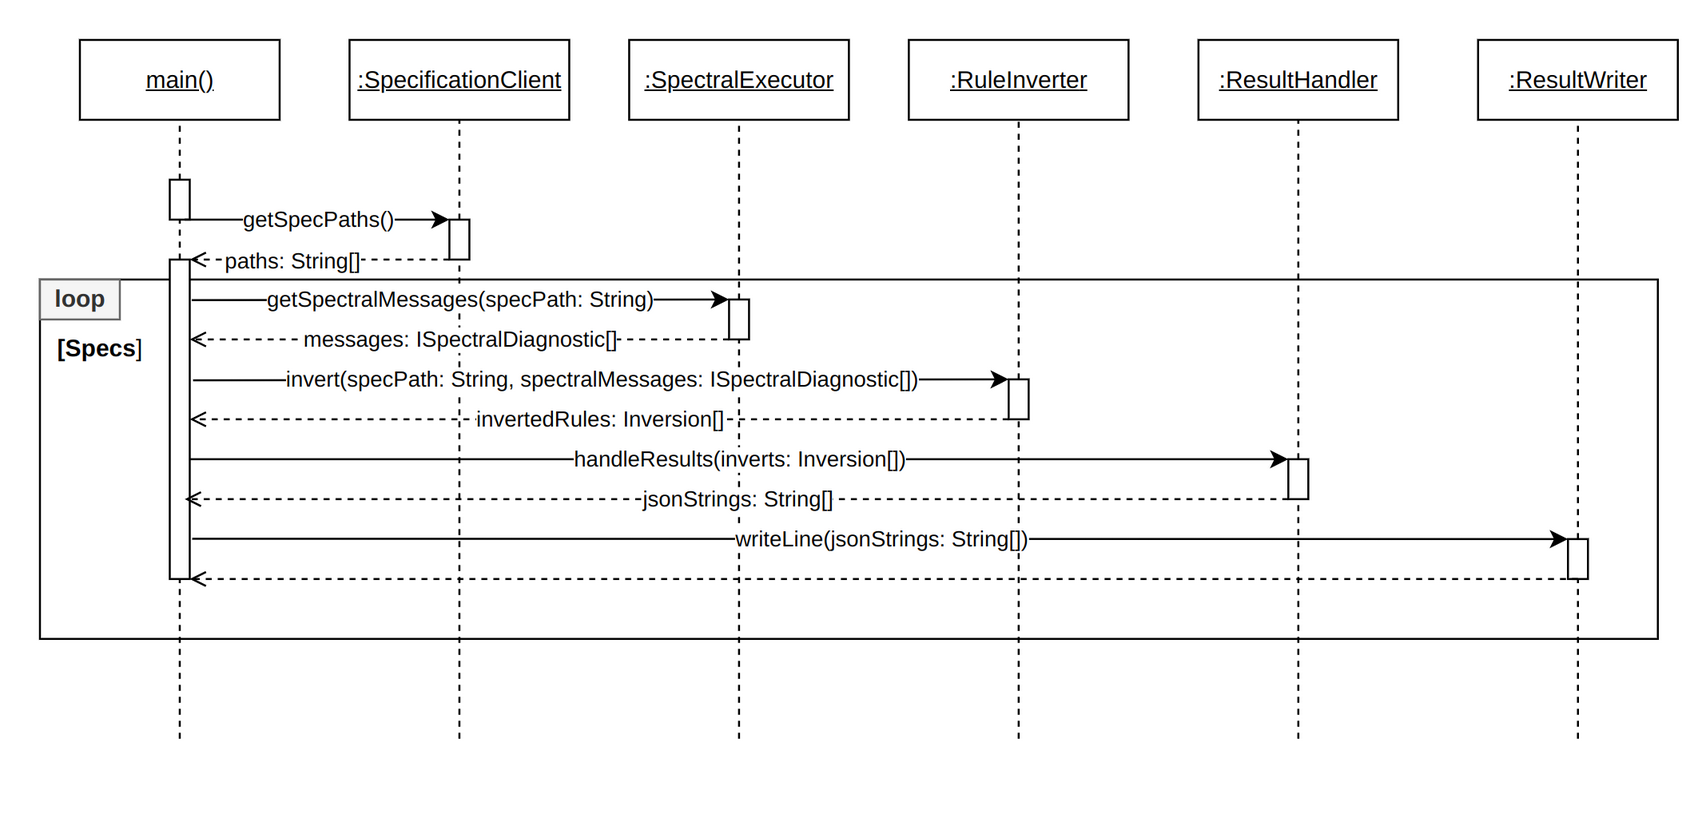
\includegraphics[width=1\linewidth]{img/runtimeview.png}
  \caption{Laufzeitsicht des Systems}
  \label{fig:Laufzeitsicht}
\end{figure}


\subsubsection{Verteilungssicht} \label{sec:verteilungssicht}
Die Verteilungssicht beschreibt die Laufzeitumgebung des Systems und deren Hardwarekomponenten \parencite{starke_effektive_2024}. Zudem werden die Laufzeitumgebungen der Software Komponenten dokumentiert, sowie Datenquellen und Datensenken definiert. 

Die Software, die in dieser Arbeit entwickelt wird, wird zu einem Großteil in der lokalen Entwicklungsumgebung ausgeführt. Als Ausnahme zählt die unabhängige Datenquelle von APIs.guru, die als Git Submodul\footnote{Dokumentation zu Git Submodulen: \href{https://git-scm.com/book/en/v2/Git-Tools-Submodules}{https://git-scm.com/book/en/v2/Git-Tools-Submodules}} eingebunden ist.

Software Tests und Qualitätsprüfungen wie Linter und Format Checks werden zudem in einer Integrationspipeline mithilfe von GitHub Actions\footnote{GitHub Actions: \href{https://github.com/features/actions}{https://github.com/features/actions}} auf einem Remote Server ausgeführt. Da dies keinen Einfluss auf die Funktionalität der Software hat, ist dieser Schritt nicht in der Verteilungssicht modelliert.

\newpage
\begin{figure}[htbp]
  \centering
  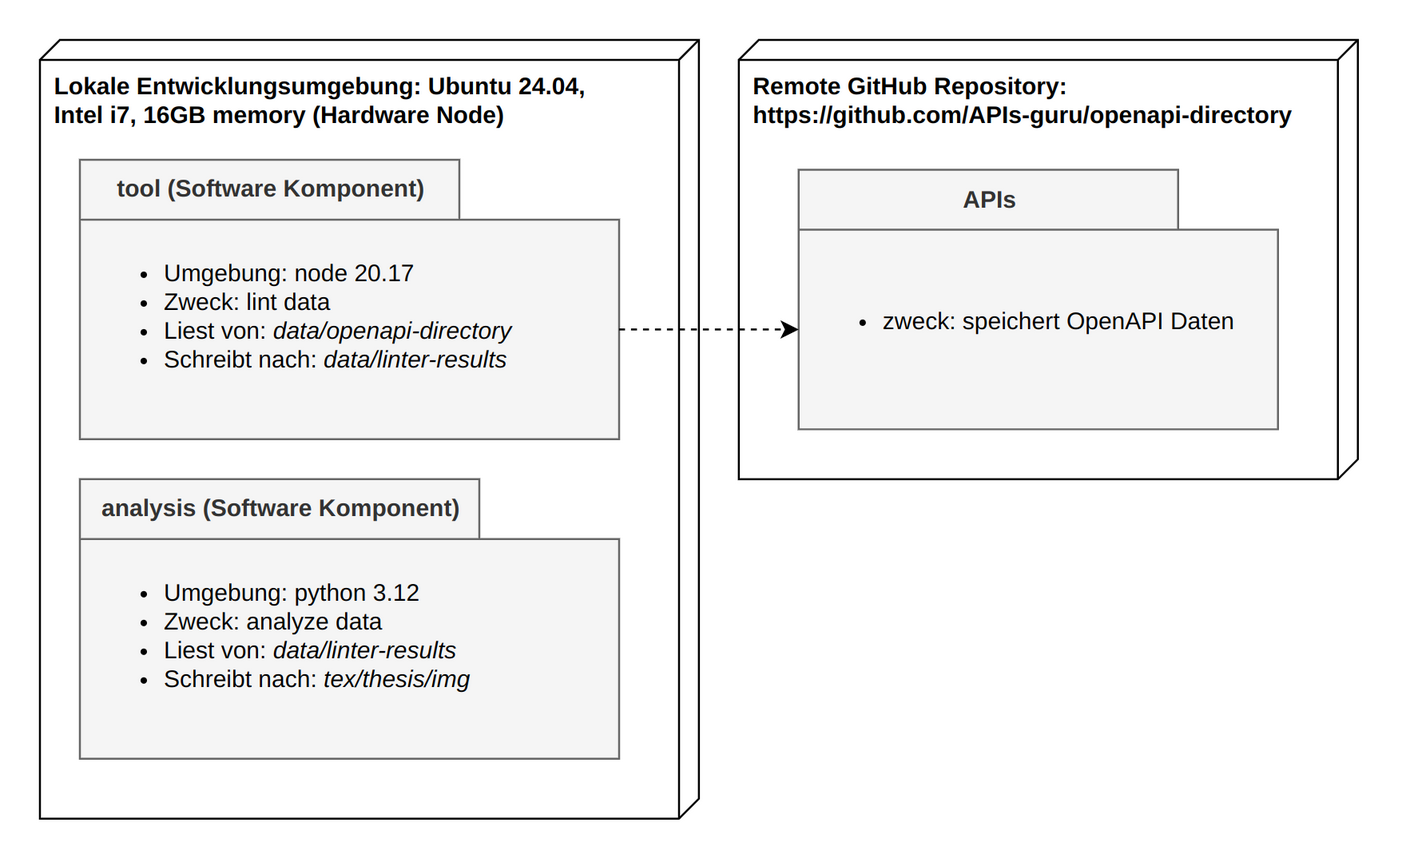
\includegraphics[width=1\linewidth]{img/deploymentview.png} \caption{Verteilungssicht des Systems}
  \label{fig:Verteilungssicht}
\end{figure}


\subsection{Datenanalyse} \label{sec:datenanalyse}
\label{chapter:dataanalysis}
Die Datenanalyse ist Teil der Software die im Rahmen dieser Arbeit entwickelt wird. Das Ziel der Datenanalyse ist es, eine datengetriebene Antwort auf die Forschungsfragen zu geben. Dazu werden statistische Methoden und Methoden des maschinellen Lernens verwendet.

In einer \acl{EDA} werden die Hauptcharakteristiken des Datensatzes aufgezeigt \parencite{tukey_exploratory_1977}. Hier können folgende Fragen beantwortet werden:

\begin{itemize}
  \item Wie viele Linterfehler wurden insgesamt ausgelöst?
  \item Wie viele Stellen gibt es, an denen Linterfehler ausgelöst werden können?
  \item Gab es Regeln, die nie Linterfehler verursacht haben?
  \item Gibt es Spezifikationen, die alle Regeln eingehalten haben?
  \item Verursacht die große Menge an Azure.com Spezifikationen eine Verzerrung in den Linterfehlern?
  \item Was sind die charakteristischen Werte der Regeln: arithmetisches Mittel, Median, Standardabweichung?
  \item Wie verhalten sich die Anzahl der geworfenen Regeln zur Größe der Spezifikation?
\end{itemize}

In einem weiteren Schritt soll die Invertierung der Regeln ausgewertet werden. Hierbei werden die Daten der geworfenen Linterfehler und der möglichen Linterfehler pro Regel verglichen. Für geeignete Regeln wird ein Boxplot über die Häufigkeit der geworfenen Regeln gezeigt.


\subsection{Priorisierung} \label{sec:methodpriorisierung}
Es werden mehrere Maße verwendet, um aus den geworfenen Linterfehlern Hinweise zu einer möglichen Gewichtung der Regeln abzuleiten. Diese Verfahren ergeben jeweils ein Scoring, zwischen 0 und 1. 1 bedeutet unabhängig vom verwendeten Maß die höchste Relevanz und 0 die niedrigste.  Am Ende werden die Werte gewichtet verrechnet, um eine Gesamtpriorisierung zu erhalten. Diese wird anschließend mit datengetriebenen Methoden in mehrere Gruppen aufgeteilt. In den folgenden Methodik Unterkapiteln wird eine Antwort auf \textbf{RQ-1} vorgestellt, die beantwortet, wie Linterregeln priorisiert werden können. 


\subsubsection{Relevanz Frequenz} \label{sec:inversedocumentfrequency}
Im Bereich des Information Retrievals und des \acs{NLP} ist die \acf{TF} - \acf{IDF} Gewichtung ein verbreiteter Score \parencite{manning_introduction_2008}. Das Maß kombiniert die \acl{TF} und die \acl{IDF}. Angewandt auf die Linterfehler, kann die \acs{TF}-\acs{IDF} Gewichtung dabei die Relevanz einer bestimmten Regel für eine Spezifikation finden. Um allgemein gültige Aussagen zur Relevanz der Regeln zu machen, eignet sich das kombinierte Maß nicht. Die \acl{IDF} eignet sich jedoch alleinstehend als Priorisierungsmaß für Linterfehler.

Wir definieren für unseren Datensatz ein Dokument als Menge von Fehlern, die zu einer Spezifikation geworfen wurden oder auch eine Zeile in der \acs{CSV} Datei mit den Linterergebnissen. Der berechnete Score basiert auf der Annahme, dass je häufiger eine Regel auf dem APIs.guru Datensatz ausgelöst wurde, desto weniger beeinflusst die Regel die Qualität der OpenAPI Spezifikation\footnote{Grundlage hierfür ist die angenommene hohe Qualität des APIs.guru Datensatzes.}. Die \acl{IDF} ist definiert durch die Anzahl an Dokumenten in einer Kollektion, die einen Term enthalten \parencite{manning_introduction_2008}. Die  Relevanz basierend auf der \acl{IDF} wird wie folgt definiert:

\[
\text{Relevanz}_\text{Frequenz}(r) = 
\begin{cases}
1&\text{, wenn } 0 = \sum_{i=1}^{n}vorkommen(r, i) \\
\frac{1}{\sum_{i=1}^{n}vorkommen(r, i)}&\text{, sonst}.
\end{cases}
\]

Die Relevanz einer Regel die nie ausgelöst wird, wird hoch priorisiert. Die Relevanz einer Regel, die nie ausgelöst wird und einer Regel, die ein Mal ausgelöst wird, ist gleich 1.

\[
vorkommen(r, s) = 
\begin{cases} 
1&\text{, wenn die Spezifikation } s \text{ die Regel } r \text{ ausgelöst hat}, \\
0&\text{, sonst}.
\end{cases}
\]


\subsubsection{Relevanz Diversität} \label{sec:diveritätsscoring}
Das zweite Priosierungsmaß soll ausschließen, dass Spezifikationen mit niedriger Qualität die Ergebnisse beeinflussen. Die Annahme ist, dass solche Spezifikationen über alle Regeln hinweg viele Fehler auslösen. Damit beeinflussen diese Relevanz der mit $\text{Relevanz}_\text{Frequenz}$ berechneten Werte.

Es wird davon ausgegangen, dass nicht intendierte Linterfehler einzigartig sind. Mit \acs{IDF} werden vertikal in der Matrix über Spezifikationen und Linterregeln einzigartige Fehler hoch priorisiert. Um auch horizontal in der Matrix einzigartige Fehler zu identifizieren, wird eine zweite Methode verwendet. Mit dieser Methodik soll die Diversität des Auslösemusters einer Regel eingefasst und in ein Priorisierungsmaß eingebettet werden.

Um solche Diversität der Regeln zu berechnen, kann die Ähnlichkeit des Auslösemusters zwischen Regeln berechnet werden. Die Spalten des Datensatzes, die das Vorkommen der Regeln dokumentieren, können als Binärvektoren interpretiert werden. Zur Bestimmung der Ähnlichkeit von Binärvektoren kann das \textit{Jaccard} Ähnlichkeitsmaß verwendet werden \parencite{mehrotra_anomaly_2017}.

\[
Jaccard(A,B)=\frac{\vert A \cap B \vert}{\vert A \vert + \vert B \vert - \vert A \cap B \vert}
\]

Je weniger das Auslösemuster einer Regel dem der anderen ähnelt, desto höher wird die Regel priorisiert. Die gemittelte Ähnlichkeit einer Regel zu allen anderen Regeln ist der finale Wert. Es wird die Relevanz basierend auf der Triggerdiversität definiert:

\[
\text{Relevanz}_\text{Diversität}(r) = (\frac{1}{n} \sum_{i=1}^{n} 1- Jaccard(r, r_i))
\]

\subsubsection{Kombination der Verfahren} \label{sec:kombinationderpriorisierungen}
Um die Werte der beiden Priorisierungsmaße zu vereinigen, wird eine gewichtete Summe verwendet. So lässt sich eine Gesamtpriorisierung der Regeln festlegen. Relevante Regeln haben höhere Werte und weniger relevante Regeln haben niedrige Werte.

Es wird davon ausgegangen, dass die Einordnung der Regeln in Schweregrade \texttt{hint}, \texttt{warn} und \texttt{error} eine Entwicklereinschätzung der Relevanz der Regeln abbildet. Um diese Einschätzung zu berücksichtigen, wird versucht die Koeffizienten $\alpha$ und $\beta$ so zu setzen, dass Regeln, die im Spectral \acs{OAS} Regelwerk den Schweregrad \texttt{error} haben eine hohe Priorisierung haben und jene mit dem Schweregrad \texttt{hint} eine niedrige Priorisierung haben.

\[
\text{Relevanz}_\text{total} = \alpha * \text{Relevanz}_\text{Frequenz} + \beta  * \text{Relevanz}_\text{Diversität}
\]

Die berechneten Werte geben Antwort auf \textbf{RQ-2} (Wie können relevante Linterregeln priorisiert werden).


\subsubsection{Clustering} \label{sec:clustering}
Spectral verwendet drei Schweregrad Level für die Regeln des Spectral \acs{OAS} Datensatzes (\texttt{hint}, \texttt{warn}, \texttt{error}) siehe auch Abbildung \ref{tab:OASRules}. Zur Beantwortung von \textbf{RQ-3} (Welche Linterregeln können empfohlen werden) soll ein Clustering der Regeln in drei Relevanzklassen erfolgen, die den Schweregraden des Spectral Linters entsprechen. Die Regeln sollen anhand ihrer Priorisierung in drei Partitionen eingeteilt werden. Dafür eignet sich der k-means Clustering Algorithmus \parencite{bishop_pattern_2006}. Das Ziel des k-means Algorithmus ist, einen Datensatz in k Partitionen zu teilen, sodass die Summe der quadrierten Abweichungen von den Clustermittelpunkten minimal ist \parencite{bishop_pattern_2006}.

Hierfür werden die mit Koeffizienten gewichteten priorisierten Werte als Vektoren verwendet. Die zwei verwendeten Priorisierungsmaße sind Dimensionen für die Partitionsidentifikation. Für k wird die Anzahl der Spectral Linter Schweregrade gewählt.

Für die Implementierung des Algorithmus wird die Pythonbibliothek sklearn\footnote{Dokumentation: \href{https://scikit-learn.org/1.5/modules/generated/sklearn.cluster.KMeans.html}{https://scikit-learn.org/1.5/modules/generated/sklearn.cluster.KMeans.html}} verwendet. Für die zufällige Initialisierung der drei Cluster Centroiden wird ein fester random state spezifiziert, um Reproduzierbarkeit zu garantieren.


\subsection{Validität der Methode} \label{sec:validitätdermethode}
In diesem Kapitel wurde die Methode vorgestellt, mit der die Forschungsfragen dieser Arbeit beantwortet werden. Abschließend wird erläutert, welche Einschränkungen die Anwendung dieser Methode hat.

Die Methodik zur Beantwortung der Forschungsfragen in dieser Arbeit geht von einer hohen Qualität der Daten im OpenAPI Directory von APIs.guru aus. Diese Annahme kann aufgrund der Verwendung des OpenAPI Directory in mehreren wissenschaftlichen Quellen \parencite{bogner_restruler_2024} \parencite{serbout_apistic_2024} getroffen werden. Die Qualität des OpenAPI Directory wird dort spezifisch erwähnt. \glqq Aufgrund des kuratierten Inhalts enthält es hochqualitative, valide und einzigartige Spezifikationen, da nicht verlässliche Quellen herausgefiltert werden\grqq{}\footnote{Übersetzt aus dem Englischen} \parencite{serbout_apistic_2024}. \glqq Diese Definitionen variierten stark in der Größe und deckten eine große Anzahl an Themen ab: von offiziellen Cloudanbieter \acs{API}s von Firmen wie Amazon und Microsoft bis zu Museums und Regierungs \acs{API}s. Nur in wenigen Fällen lagen mehrere Versionen der gleichen \acs{API} vor, was zur Varianz beiträgt. Die Dokumente nutzen OpenAPI Konzepte wie Components oder Responses sehr unterschiedlich, was sie sehr verschieden macht. Dies qualifiziert sie als ideale Testbasis für unsere Implementierung ...\grqq{}\footnote{Übersetzt aus dem Englischen} \parencite{bogner_restruler_2024}.

Die \acl{IDF} wird als Priorisierungsmaß verwendet, da Linterregeln, die auf Spezifikationen hoher Qualität häufig ausgelöst werden, keinen Einfluss auf die Qualität des Dokumentes haben.
Mit Daten schlechter Qualität ist diese Bedingung für die Nutzung von \acs{IDF} als Priorisierung nicht mehr gegeben.

Um dieses Risiko abzumildern wird mit der Diversität der triggernden Spezifikationen ein zweites Priorisierungsmaß eingeführt. Dies soll den Effekt von Spezifikationen schlechter Qualität auf die Gesamtpriorisierung abmildern.

Um Risiken durch in der Funktionalität fehlerhafte Software zu minimieren wird der Code, der im Rahmen dieser Arbeit entwickelt wurde, mit Unit-Tests getestet und es wird ein Coverage Gate von 80 \% Funktionsabdeckung technisch sichergestellt. Dennoch kann so die Korrektheit des Programmcodes nicht nachgewiesen werden. \glqq Das Testen von Programmen kann die Existenz von Fehlern zeigen, aber niemals deren Nichtvorhandensein\grqq{} \parencite{dijkstra_notes_1970}.